\documentclass{article}
\usepackage[utf8]{inputenc}
\usepackage{indentfirst}
\usepackage{amsmath}
\usepackage{graphicx}
\usepackage{subcaption}
\usepackage{placeins}

\title{Can a Shallow Ice Approximation Model be Used to Model the Water Output of Alpine Glaciers?}
\author{}
\date{}

\begin{document}

\maketitle

\section*{Abstract}

\section{Introduction}
\subsection{Importance of glacial melting in mountain hydrology}
Glacial melting plays a significant role in the hydrology of mountain catchment areas as shown in Fountain and Tangborn, 1985. Accurately 
capturing glacial dynamics with numerical models is important for understanding how water sources in high mountain catchments will evolve. 
The runoff produced by glaciers, especially later in the summer months, is a major contributor to stream flow. Without the runoff from the 
glaciers, the rivers would be even lower during the driest summer months as shown in Figure 1.

As glaciers melt and retreat, the change in mass takes the form of meltwater. This meltwater affects communities downriver in a variety of 
ways. For instance, many communities rely on these rivers as a water source for drinking and irrigation.  

\begin{figure}[h]
    \centering
    \begin{subfigure}[b]{0.45\textwidth}
        \centering
        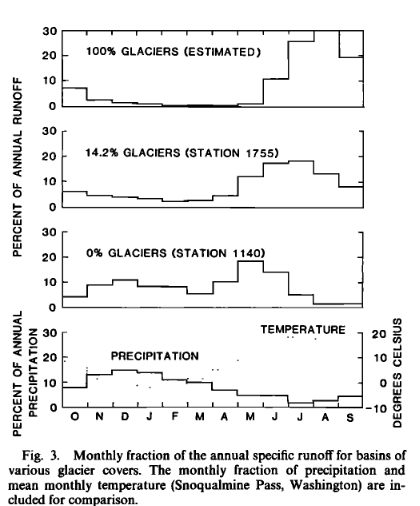
\includegraphics[width=\textwidth]{Plots/fountain_1985_fig3.png}
        \caption{Monthly fraction of the annual runoff for basins of various glacier cover.}
        \label{fig:subfig1}
    \end{subfigure}
    \hfill
    \begin{subfigure}[b]{0.45\textwidth}
        \centering
        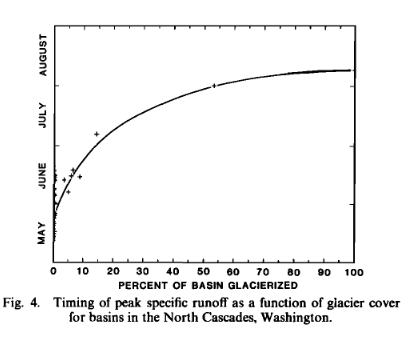
\includegraphics[width=\textwidth]{Plots/fountain_1985_fig4.png}
        \caption{Timing of peak specific runoff as a function of glacier cover.}
        \label{fig:subfig2}
    \end{subfigure}
    \caption{Figures 3 and 4 from Fountain and Tangborn (1985) showing how the percent of basin glacierized delays the peak runoff time of the basin.}
    \label{fig:main_figure}
\end{figure}
\FloatBarrier
\subsection{Role of numerical modeling in understanding glacial runoff}
One of the best ways to find out how glaciers will affect the stream flow of rivers in the glacier basin is by using computer models to 
approximate the water discharge of the glaciers. Scientists have been using computers to model glaciers for several decades, such as this 
paper by Iken A, 1981. As computational resources have grown, these models have grown in complexity and resolution leading to very 
computationally expensive models, meaning that they take a lot of computing power to run. Many of these Advanced Ice Sheet Models (AISMs) 
use equations such as the 3-dimensional Stokes equations (Larour et al., 2012) to model the complicated ice dynamics of these glaciers.  
\subsection{Challenges in computational modeling of glaciers}
AISMs are numerically very sophisticated; these models are also not very intuitive and often take a while to learn how to run. The advantage 
of AISMs is that they do a particularly good job of modeling ice dynamics. For some glaciers such as marine calving glaciers, accurate ice 
dynamics are crucial to accurately model them, as shown in Amaral et al., 2020. However, modeling glaciers in 3-dimensions is often 
unnecessary. If we can use simpler models, such as the Shallow Ice Approximation (SIA) model, to calculate the water runoff of small 
mountain glaciers in locations such as the Alps, then we can run these models over more glaciers and larger areas, and it is easier to 
incorporate them into larger hydrology models. 

\section{Literature Review}
\subsection{Prior research on SIA vs. Stokes models}
    As shown in Le Meur et al., 2004, there are significant differences in computational time between a SIA model and a Stokes model. When 
computing the free surface and associated velocity field, the SIA model took 1 minute of CPU time, whereas the Stokes model took 2 hours. 
This disparity grew even larger for 3D models. The authors show that there are some instances where SIA models do significantly worse than 
Stokes models, such as glaciers on steep slopes and glaciers in steep, narrow valleys because SIA models only approximate the Stokes 
equations. One of these approximations is to ignore horizontal stress gradients. This can cause a SIA model to deviate from a Stokes model 
significantly in predicted glacier flow and expansion. In one example, the resulting SIA model can have an upper free surface that is 
15--20\% greater than the Stokes model and velocities up to a factor of 2 greater (Le Meur et al., 2004). In the 2D model, the bed 
characteristics and slope become the limiting factor of the SIA model; Le Meur et al., 2004 note that the maximum velocity ratio of their 
SIA and Stokes models goes from 1.9 in a 3D model to 1.3 in a 2D model, which will differ depending on model configuration, but it tends to 
indicate that the horizontal stress gradients played a large part in this error. They found instances in which the SIA models performed well 
compared to Stokes models---particularly large flat glaciers with relatively free edges. One thing to note about this comparison study is 
that the authors are looking at the shape, area, and velocity profile of the glacier, whereas this study will focus on the water output 
(surface mass loss) of the glacier.
\subsection{Using SIA models to model alpine glaciers}
    There are several papers, such as Le Muer et al., 2003 and Kessler et al., 2006, that use an SIA model for alpine glaciers. The consensus 
from those papers is that SIA models only work well on alpine glaciers with a low aspect ratio, defined as the thickness-to-extent ratio in 
Le Muer et al., 2004. The glacier used by this study will have a low aspect ratio and therefore a SIA model should work well to model it.
\subsection{Using SIA models to model water runoff from glaciers}
    Additionally, there is precedent for using a SIA-Mass Balance model for modeling water runoff from glaciers (Naz et al., 2014). They used 
the SIA model to approximate the ice dynamics and a mass balance model to approximate the accumulation and ablation patterns on the glacier. 
As shown in their paper, the SIA model was able to accurately predict the glacier, and the coupled hydrological model was able to predict 
the stream flow accurately---only overestimating the July flow by an average of 13\% and underestimating the August and September flow by an 
average of 2\%.

\section{Thesis Statement}
%Fix this to reflect the OGGM comparison
How much do ice dynamics affect the model result when modeling small mountain glaciers for mass balance? I theorize that if using a simple 
1-dimensional SIA-Mass Balance model on small mountain glaciers (with a low aspect ratio) in the Alps, the mass balance profile will have a 
much larger effect on the output of the model and its overall accuracy than the modeled ice dynamics. The results of the SIA-Mass Balance 
model and the Stokes model will be compared to the actual stream flow data to verify this hypothesis.
\subsection{Study Site}
\textbf{\large South Cascade Glacier, Washington State}

In this study, I will focus on modeling the South Cascade Glacier in the North Cascades region of Washington State. South Cascade Glacier is 
roughly 1.79 square kilometers, has a mean elevation of roughly 1900 meters, faces North, has an average slope of 12.8 degrees (need new 
source), an average thickness of ??? meters, and a maximum thickness of ???? meters (GlaThiDa Consortium, 2020). The glacier is small, not 
overly steep, and has a low aspect ratio such that a shallow ice approximation (SIA) model should be able to accurately represent its ice 
dynamics. On the other hand, the glacier is large enough to exhibit some movement and produce a measurable amount of runoff throughout the 
year. It is also one of the USGS Benchmark glaciers which means there is a large amount of data on it available such as temperature, 
precipitation, mass balance, front variation, and thickness change. In 1992 a stream gauge was installed just below the glacier which allows 
one to calculate the runoff from the glacier. 
\begin{figure}[h!]
    \centering
    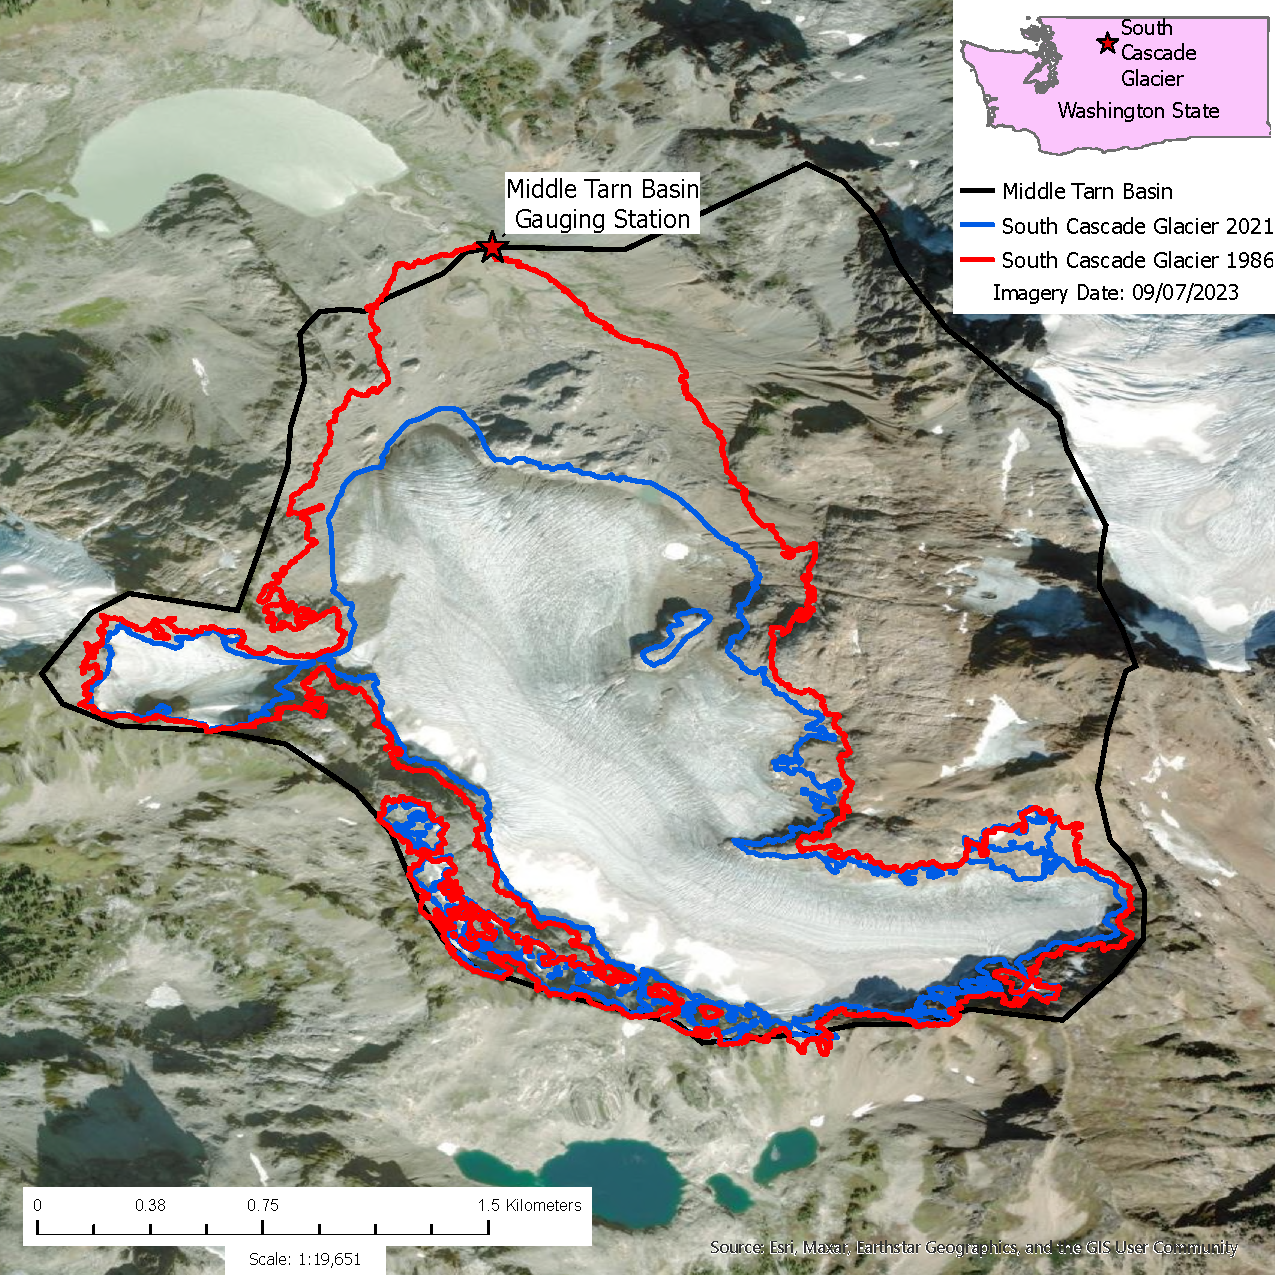
\includegraphics[width=\textwidth]{Plots/SouthCascadeGlacierMap.pdf}
    \caption{Map of the South Cascade Glacier in the North Cascades of Washington.}
    \label{fig:south_cascade_glacier}
\end{figure}
\FloatBarrier
\section{Methods}

\subsection{Model Development}
\subsubsection{Model Overview}
The model is a one-dimensional shallow ice approximation (SIA) model coupled with a degree day mass balance model. The structure of the model is
\begin{enumerate}
    \item SIA model for ice dynamics
    \item Degree day and precipitation mass balance model
    \item Degree day and precipitation snow model
\end{enumerate}

There are two main sections to the model run, spinup and run. The spinup section of the model runs for 500 years and aims to replicate the 
state of the glacier in 1984 when weather data becomes readily available. This section uses the simple mass balance equation below
\begin{equation}(\text{glacier elevation}-\text{ELA})*\text{gamma}/365.25\end{equation}
This calculates the mass balance in meters per day. When the spinup hits the year 1900 the ela is shifted up by 50 meters to simulate the 
retreat state of the glacier. 

The run portion of the model runs from 1984-2024 and is described below.

\subsubsection{Ice Dynamics}
\paragraph{SIA Model}

The SIA model is a one-dimensional model that uses the shallow ice approximation to approximate the ice dynamics of the glacier. This model 
calculates the one dimensional ice flux of the glacier using equation 1. 
\begin{equation}Q=\frac{2A}{n+2}(p_{ice}g|\frac{\partial z_s}{\partial x}|)^n\frac{H^5}{5}\end{equation}
Where $Q$ is the ice flux, $A$ is the flow rate factor, $n$ is the flow law exponent, $p_{ice}$ is the density of ice, $g$ is the acceleration
due to gravity, $\frac{\partial z_s}{\partial x}$ is the slope of the glacier, and $H$ is the thickness of the glacier. This model works by 
creating an array of bins that represent the glacier. The model then calculates the ice flux of each bin and uses that to create the flow of 
ice in the model. 
\paragraph{Assumptions}

The SIA equations make several assumptions. First, the equations neglect longitudinal stress, ice only flows downhill. Second, the equations 
also assume that there is no basal sliding of the glacier. Third, the equations only use gravity as the driver of ice flow; they ignore other 
forces such as lateral and basal stress. Fourth, this set of equations assumes that the horizontal dimensions of the modeled glacier are much 
larger than the vertical dimensions.

The South Cascade Glacier was chosen because of some of these assumptions, it's horizontal dimensions are significant larger than its vertical 
dimensions, and it is not a steep or fast flowing glacier, allowing the SIA assumptions to hold.

\subsubsection{Model Setup}
The model relies on a variety of input data in order to run. Besides the temperature and precipitation data described below the model also 
needs a bed topography to run. This is input into the model as a csv with a latitude, longitude and elevation columns. The data in this model 
is from (reference). The model loads the data an interpolates it across the number of cells into the model to create a topography variable to a
act as the bed surface for the glacier. 

\subsubsection{Mass Balance Model}
The mass balance of the glacier is calculated using temperature and precipitation data from the Diablo Dam weather station at 272m. The 
temperature at the glacier is calculated by using a month-specific lapse rate. This month-specific lapse rate was empiraclly calculated using
data from the Diablo Dam weather station and the South Cascade Glacier weather station at 1830m from 2010-2018. The precipitation at the 
glacier is calculated by multiplying the precipitation at the Diablo Dam weather station by the precipitation conversion factor of 1.58 
(reference). The ablation of the glacier is calculated by using a combination of an ice melt factor and a snow melt factor. Above the ELA the 
ablation is calculated by the equation
\begin{equation}\text{ablation}=T*\text{snow melt factor}\end{equation}
Below the ELA the ablation is calculated by the equation
\begin{equation}\text{ablation}=T*(\text{snow melt factor}+((\text{ELA}-\text{elevation})/(\text{ELA}-\text{minimum(elevation)}))*$$
$$(\text{ice melt factor}-\text{snow melt factor}))\end{equation}
The result of this equation is the snow melt factor being used at the ELA and a linear increase in the melt factor until it hits the ice melt 
factor at the base of the glacier. 
The accumulation of the glacier is calculated using a similar linear equation that increases with time.
\begin{equation}\text{accumulation}=p*\alpha*(\text{start accumulation}+((\text{year}-1984)/(2024-1984))*$$
$$(\text{start accumulation}-\text{end accumulation}))\end{equation}
This resuls in the accumulation increasing with time until it hits the end accumulation at 2024. 

\subsubsection{Snow and Rain Model}
The snow melt model uses precipitation and temperature data to melt and accumulate snow. This model uses 14 elevation bins and keeps track 
of the snow depth in each bin. Each elevation bin has a corresponding area that represents the area of the basin in the bin's elevation range. 
The equation below is used to calculate the change in snow depth per timestep 
\begin{equation}\text{snow depth} += 
\begin{cases} 
  p*\alpha & \text{if } T \leq 0,\\
  -\text{minimum}((s*T),\text{snow depth}) & \text{if } T > 0
\end{cases}\end{equation}
Where $p$ is the precipitation, $\alpha$ is the precipitation conversion factor, $s$ is the snow melt factor, and $T$ is 
the temperature. The snow melt is constrained so that there cannot be more melt than there is snow. The rain is simply modeled by $p*\alpha$ 
for positive temperatures

The total volume of snow is calculated by the equation
\begin{equation}\text{snow melt volume}=(s*T)*(\text{area of bin}-\text{area of glacier})\end{equation}
This give us the total volume of snow melting off the glacier. The glacial melt is calculated elsewhere. The volume of rain is calculated by
\begin{equation}\text{rain volume}=p*\alpha*(\text{area of bin})\end{equation}
This calculates the rain for the whole basin, assuming that any rain that falls off the glacier runs off immediately.

\subsubsection{Glacial Melt Model}
The glacial melt model uses the mass balance of the glacier to calculate how much volume the glacier is losing. The volume of runoff from the 
glacier per timestep is calculated by the equation
\begin{equation}\text{glacial melt volume}=(\text{mass balance}<0)*\text{area of glacier}\end{equation}
\subsection{Data Used for Model}
The temperature and precipitation data used for the model is from the Diablo Dam weather station at 272m. The data is available from 1984-2024 
and is only missing XXXX days in that time period (reference). The glacier area data used in the model is from the USGS (reference). The basin 
area data was calculated using a DEM from the USGS and the basin outline shown in figure XXXX.

\subsubsection{Model Calibration}
The spinup initial ela, ela shift and gamma were manually optimized to match the glacier extent in 1984. 

The ice and snowmelt factors were calibrated using summer mass balance data available from the USGS from 1984-2024. I used the minimize 
function using the Nelder-Mead method from the scipy library to minimize the mean squared error between the model and the data. The 
accumulation factors were calculated using the same methodology for the winter mass balance data available from the USGS from 1984-2024.

The avalanche percentage was optimized using the same methods as the mass balance variables, but instead of a mean squared error being 
minimized, the mean of the snow depth over the period 1984-2024 was minimized. 

\subsubsection{Model Comparison}
\paragraph{Running OGGM Model for the Same Glacier}

The OGGM model was run using the run\_with\_hydro task from the oggm library. This model run used CMIP5 historical temperature and 
precipitation data to model the hydrology of the glacier from 1984-2019. Using the output of this model I was able to calculate the total 
runoff from the glacier using the melt\_on\_glacier\_monthly, snowmelt\_on\_glacier\_monthly and liq\_precip\_on\_glacier\_monthly variables. 
The MSE of the OGGM model and my model is 5.31\% and the MSE of the OGGM model and the measured runoff data is 3.93\%.

\paragraph{Validation Using Real-World Streamflow Data }

The calculated runoff of the SIA-Mass Balance model was validated using measured streamflow data from 1992-2007. This data was measured using 
a stream gauge located just below the glacier. The data is in units of mm per day averaged over the basin area (4.46$\text{km}^2$). I 
converted this to cubic meters per day by divinding each value by 1000 and multiplying by the basin area in square meters. None of the input 
parameters to the model were specifically tuned to match the streamflow data. The melt factors were tuned to match the yearly summer mass 
balance, the accumulation factors were tuned to match the yearly winter mass balance, the avalance percentage was tuned to minimize the 
average snow depth over the model run, the lapse rates were empirically calculated using data from the Diablo Dam weater station and a weather station 
at 1830 meters next to the South Cascade glacier, and the precipitation conversion factor was obtained from (reference). The model was able 
to calculate the runoff from the whole basin (snowmelt, glacier melt and rainfall) from 1984-2024 with a mean squared error of 1.41\%.

\section{Expected Results}
\subsection{Accuracy of SIA}
\subsection{Accuracy of OGGM}
\subsection{Comparison of Accuracy}

\section{Implications of Research}
\subsection{Importance of Simplified Ice Dynamics in Numerical Glacier Modeling}
These results show that complicated and computationally intensive mass balance, melt and ice dynamics are not required to accurately model the 
runoff from small mountain glaciers. This means that we can use much simpler and less computationally intensive models such as the ones used 
in this paper to model the runoff from mountain glaciers over a much larger area. The modeling techniques used in this paper could easily be 
scaled to a much larger region if mass balance is available to tune the input parameters. I would hypothesize that the input parameters used 
in my model of the South Cascade Glacier could be used for a much larger model over a similar region as almost all of the input parameters are 
climate dependet, but this is a topic for another paper. 
\subsection{Applications}

\section{Discussion}
\subsection{What Worked}
\subsection{What Didn’t Work and Why}
\subsection{What Can Be Improved}

\section{Conclusion}
\subsection{Summary of Results}
\subsection{Conclusion of Model Accuracy}

\section{References}
% (Insert references here.)

\end{document}
